\section{Aufbau und Durchf\"uhrung}
\label{sec:Durchfuehrung}
Die Apparatur ist in Abbildung \ref{fig:aufbau} schematisch skizziert.
\begin{figure}[h]
	\centering
	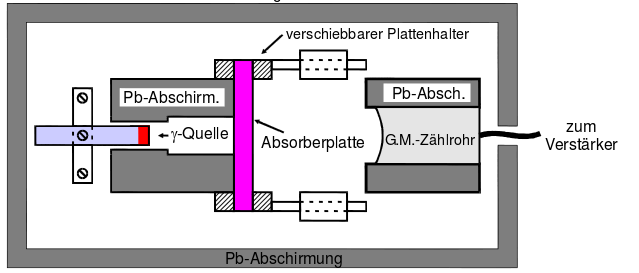
\includegraphics[width=\textwidth]{Bilder/aufbau.png}
	\caption{Schematischer Aufbau des Zählwerks \cite{skript}}
	\label{fig:aufbau}
\end{figure}
In einem Bleigehäuse, das der Abschirmung von Strahlen dient und damit zur Arbeitssicherheit gehört, befindet sich ein Geiger-Müller-Zählrohr.
Dies ist auf den Detektorbetrieb eingestellt und unterscheidet somit nicht die Art der Strahlung.
Angeschlossen an ein zeitgesteuertes Zählwerk kann mit dem Zählrohr die Strahlung gemessen werden, die eine Blende durchdringt.
Auf einer Schiene befinden sich hierfür in Reihenfolge das radioaktive Präparat, eine austauschbare Blende und die Messeinrichtung.
Weiterhin befindet sich unmittelbar um das Zählrohr ein weiteres Bleigehäuse, das dazu dient, die Nullstrahlung abzuschirmen und damit den statistischen Fehler zu lindern.

Aufgrund der natürlichen Hintergrundstrahlung ist ein Messergebnis nicht ausschließlich auf den Zerfall des Präparats zurückzuführen, obwohl der zusätzliche Bleischirm angelegt wird.
Um aus den abgelesenen Messwerten Aussage über das Präparat zu treffen, wird vor Beginn des Experiments für $\SI{750}{\second}$ ohne Blende und ohne Präparat die Nullstrahlung gemessen und diese Strahlung bei der Auswertung berücksichtigt.
Es folgen zwei grundlegende Messungen: die erste an einem \texorpdfstring{$\gamma$}{Gamma}-Strahler, die zweite an einem \texorpdfstring{$\beta$}{Beta}-
Strahler.\\
Es wird die \texorpdfstring{$\gamma$}{Gamma}-Absorptionskurven von Eisen und zusätzlich Blei aufgenommen.
Mittels Ausgleichsrechnung wird der Absorptionskoeffizient $\mu$ und die Größe $N_0$ bestimmt (vgl. Abschnitt \ref{sec:absorp}, Gleichung \eqref{eq:Absorptionsgesetz}). 
Als Strahlungsquelle wird das Nuklid 137-Cäsium verwendet.
Die erhaltenen Werte für Absorptionskoeffizient $\mu$ werden mit den in der Theorie vorhergesagten Werten verglichen und somit erschlossen, 
welcher der vorgestellten Absorptionsmechanismen im vorliegenden Fall auftrat.

Es wird die \texorpdfstring{$\beta$}{Beta}-Absorptionskurve von einem Aluminiumabsorber aufgenommen und 
mithilfe der Reichweitenbestimmung die maximale Energie der \texorpdfstring{$\beta$}{Beta}-Strahlung abgeschätzt.
Hierzu findet das Präparat 99-Technetium Verwendung, das durch 10 Aluminiumblenden verschiedener Dicke hindurchstrahlt.
Für jede Blende wird der Anzahl der Zerfälle in $\SI{350}{\second}$ oder in $\SI{500}{\second}$ bestimmt.
